\documentclass{pset}

\renewcommand{\hmwkTitle}{3rd\ week\ hw}
\renewcommand{\hmwkDueDate}{February 12, 2014}
\renewcommand{\hmwkClass}{Measure Theory}
\renewcommand{\hmwkClassTime}{Chapter 2}
\renewcommand{\hmwkAuthorName}{}

%
% Title Page
%

\title{
    \vspace{2in}
    \textmd{\textbf{\hmwkClass:\ \hmwkTitle}}\\
    \normalsize\vspace{0.1in}\small{Due\ on\ \hmwkDueDate\ at 3:10pm}\\
    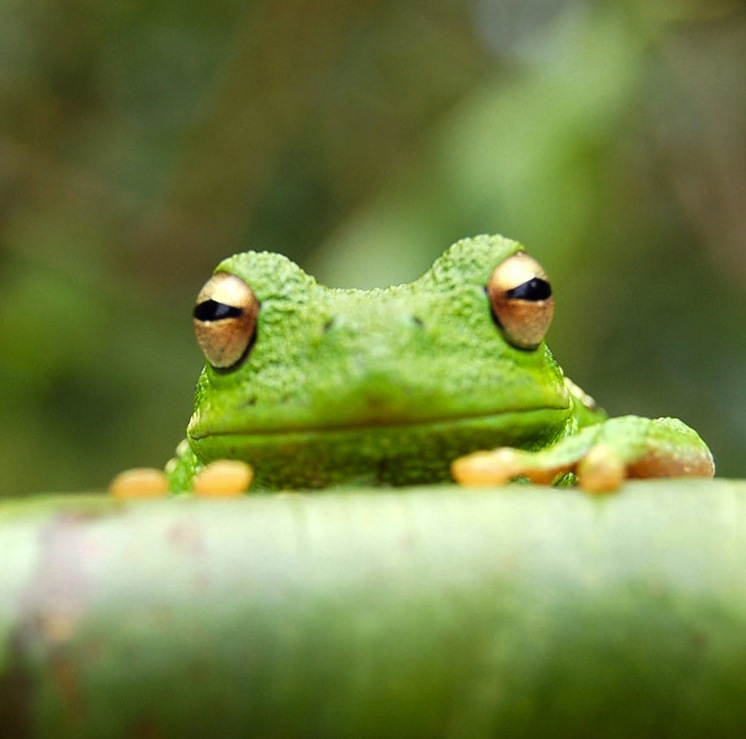
\includegraphics[scale=0.2]{frog} \\
    \vspace{0.1in}\large{\textit{\hmwkClassTime}}
    \vspace{3in}
}

\author{\hmwkAuthorName}
\date{}

\renewcommand{\part}[1]{\textbf{\large Part \Alph{partCounter}}\stepcounter{partCounter}\\}

% Integral dx  
\newcommand{\dx}{\mathrm{d}x}

\begin{document}

\maketitle

\pagebreak 

\begin{problem}
    \begin{enumerate}[label=\alph*.]
        \item 
        \begin{enumerate}[label=$\bullet$]
            \item if $f$ is infinite on a set $E$ with positive measure then
            \[
                \int f \dd \mu \geq \int N\scalebox{1.25}{$\chi$}_E \dd \mu=N\cdot\mu(E)
            \]
            for any integer $N$ and simply letting $N\to+\i$ gives us what we want.
            \item if $f$ is simple then the theorem is trivial. For the general, due to p case there must exist an increasing sequence of simple functions $\{\phi_n\}_0^\i$ that converge to $f$ pointwise. Let $\mcl{E}_n$ be the colleciton of sets where $\phi_n$ is positive, note that $\mcl{E}_n$ is a finite collection of sets with finite measure. And it's obvious that $f$ is positive on $\bigcup_{i=0}^\i\bigcup_{E\in\mcl{E}_n}E$ and hence we're done.
        \end{enumerate}
        \item it's literally the same proof ):$<$.
        $f$ is measurable by proposition 2.11 and 2.12, and since for each $x$, $\abs{f_n(x)}\to \abs{f(x)}$ and $g_n(x)\to g(x)$ and since $\abs{f_n(x)}\leq g_n(x)$ then $\abs{f(x)}\leq g(x)$ then we have $\abs{f}\leq g$ which means $f\in L^1$. By taking real and immaginary parts it suffices to assume $f_n$ and $f$ are real valued. And since $f_n-g_n\geq 0$ and $f_n+g_n\geq 0$ we can use Fatou's lemma:
        \begin{align*}
            \int g + \int f \leq \liminf\int(g_n-f_n) \leq\liminf \int g_n + \liminf \int f_n \\
            \int g - \int f \leq \liminf\int(g_n-f_n) \leq\liminf \int g_n-\limsup\int f_n
        \end{align*}
            Therefore, $\limsup \int f_n\leq\int f\leq \liminf\int f_n$ and the result follows. 
        \item
        \begin{enumerate}[label=$\bullet$]
            \item as $n\to\i$ we see that $\frac{\sin(\frac{x}{n})}{(1+\frac{x}{n})^n}\to 0$, $\frac{1}{(1+\frac{x}{n})^n}\to e^{-x}$ and we have
            \[
                \int_0^\i\frac{1}{(1+\frac{x}{n})^n}\dd x=\frac{n}{n-1}\to 1 = \int_0^\i e^{-x}\dd x
            \]
            and since $\abs{\frac{\sin(\frac{x}{n})}{(1+\frac{x}{n})^n}}\leq \frac{1}{(1+\frac{x}{n})^n}$ we can use the generalized DCT to conclude that
            \[
                \lim_{n\to\i}\int_0^\i\frac{\sin(\frac{x}{n})}{(1+\frac{x}{n})^n}\dd x=\int_0^\i0\dd x = 0
            \]
            \item due to bernouli's inequality, $\frac{1+nx^2}{(1+x^2)^n}<1$ and we also have
            \[
                \lim_{n\to\i}\frac{1+nx^2}{(1+x^2)^n}=\lim_{n\to\i}\frac{n}{(1+x^2)^{n-1}}-\frac{n-1}{(1+x^2)^n} = 0
            \]
            (see baby rudin theorem 3.20) and hence we can use the DCT to get
            \[
                \lim_{n\to\i}\int_0^1\frac{1+nx^2}{(1+x^2)^n}\dd x=\int_0^1 0\dd x= 0
            \]
            \item since $\sin(x)<x$ we see that $\abs{\frac{\sin(\frac{x}{n})}{\frac{x}{n}}\cdot\frac{1}{1+x^2}}<\frac{1}{1+x^2}$ and we know that
            \[
                \int_0^\i \frac{1}{1+x^2}\dd x=[\arctan(x)]_0^\i=\frac{\pi}{2}
            \]
            and as $n\to\i$ we see that $\frac{\sin(\frac{x}{n})}{\frac{x}{n}}\cdot\frac{1}{1+x^2}\to \frac{1}{1+x^2}$ so by using DCT we see that
            \[
                \lim_{n\to\i}\int_0^\i \frac{\sin(\frac{x}{n})}{\frac{x}{n}}\cdot\frac{1}{1+x^2}\dd x =\int_0^\i \frac{1}{1+x^2} \dd x= \frac{\pi}{2}
            \]
            \item a simple $u=nx$ substitution would show us that
            \[
                \lim_{n\to\i}\int_a^\i \frac{n}{1+n^2x^2} \dd x = \lim_{n\to\i} \frac{\pi}{2}-\arctan(na)
            \]
            which is equal to
            \begin{enumerate}[label=$\bullet$]
                \item $0$ if $a>0$
                \item $\frac{\pi}{2}$ if $a=0$
                \item $\pi$ if $a<0$
            \end{enumerate}
        \end{enumerate}
    \end{enumerate}
\end{problem}

\begin{problem}
    \begin{enumerate}[label=\alph*.]
        \item Let $E_{n, k}=\{x\mid \abs{f(x)-f_n(x)}\geq \frac{1}{k}\}$. First, if you fix $k$ and let $n\to\i$ note that $\mu(E_{n, k})\to 0$ since $\int\abs{f-f_n}\to 0$.
        
        Choose $m_k$ such that $\mu(E_{N, k})<2^{-k}$ for all $N\geq m_k$ and $m_{k-1}<m_k$; we claim $\{f_{m_k}\}_{k=0}^\i$ converges to $f$ a.e. Indeed, suppose the sequence \emph{doesn't} converge pointwise at $x$, that means there exists an $\eps>0$ such that $\abs{f(x)-f_n(x)}\geq \eps$ for infinitely many $n\in\bN$ but that would mean $x\in \limsup E_{m_k}$. Now we'll be done if we prove $\mu(\limsup E_{m_k})=0$:
        \begin{align*}
            \mu(\limsup E_{m_k}) &= \mu\biggl(\bigcap_{i=0}^\i\bigcup_{k=i}^\i E_{m_k}\biggr) \\
            &= \lim_{k\to\i}\mu\biggl(\bigcup_{k=i}^\i E_{m_k}\biggr) \\
            &\leq \lim_{k\to\i}\sum_{i=k}^\i\mu(E_{m_k}) \\
            &< \lim_{k\to\i}\sum_{i=k}^i\frac{1}{2^i} \\
            &< \lim_{k\to\i} \frac{1}{2^{k-1}} = 0
        \end{align*}

        bonus: the typewriter sequence (I coincidentally came up with this on my own and I don't know if I should type it out ;-; )
        \item We're gonna prove b, c and d in one go. Pick $m_k$ such that $\int \abs{f_n-f_m}<2^{-k}$ for all $n>m\geq m_k$ and $m_{k-1}<m_k$. Put $f=f_{m_1}+\sum_{i=1}^\i f_{m_{k+1}}-f_{m_k}$, since $\sum_{i=1}^\i\int \abs{f_{m_{k+1}}-f_{m_k}}<\sum_{i=1}^\i 2^{-k}<\i$, due to the DCT, $f\in L^1(X)$ and
        \begin{align*}
            f &= f_{m_1}+\lim_{j\to\i}\sum_{i=1}^j (f_{m_{k+1}}-f_{m_k}) \\
            &= f_{m_1}+\lim_{j\to\i} f_{m_{j+1}} - f_{m_1} \\
            &= \lim_{j\to\i} f_{m_{j+1}}
        \end{align*}
        now choose a $N$ such that $\eps>2^{-N}$. So for all $m>n>m_N$ we have
        \[
            \int\abs{f_m-f_n}<\eps
        \]
        and
        \[
            \abs{f-f_n}=\lim_{j\to\i}\abs{f_{m_{j+1}}-f_n}
        \]
        and by using Fatou's lemma we have
        \[
            \int \abs{f-f_n}\leq \liminf_{j\to\i}\int \abs{f_{m_{j+1}}-f_n} < \eps
        \]
        which would prove the sequence converges to $f$ in $L^1(X)$ which would give us d, and by using a that would give us both b and c.
    \end{enumerate}
\end{problem}

\begin{problem}
    Since simple functions are dense in $L^1(X)$ it suffices to prove that for all $\eps>0$ and all simple functions $\phi\in L^1(X)$ there exists a function $f\in C_c(X)$ such that \(\int \abs{f-\phi}<\eps\). 
    
    Let $\sum z_j\Chi_{E_j}$ be the standard representation of $\phi$. For each $j$, we can find sets $K_j\subset E_j\subset O_j$ where $\mu(O_j\setminus E_j)<\frac{\eps}{3 \cdot 2^{j}\abs{z_j}}$ and $\mu(E_j\setminus K_j)<\frac{\eps}{3 \cdot 2^{j}\abs{z_j}}$ and using urysohn's lemma there must exist a continuous function $f_j$ such that $\Chi_{K_j}<f<\Chi_{O_j}$ and hence we have
    \begin{gather*}
        \abs{f_j-\Chi_{E_j}} \leq \abs{\Chi_{O_j}-f_j}+\abs{\Chi_{O_j}-\Chi_{E_j}} \\
        \abs{f_j-\Chi_{E_j}} <\big(\Chi_{O_j}-\Chi_{K_j}\big)+\big(\Chi_{O_j}-\Chi_{E_j}\big) \\
        \abs{f_j-\Chi_{E_j}} <\big(\Chi_{O_j}-\Chi_{E_j}\big)+\big(\Chi_{E_j}-\Chi_{K_j}\big)+\big(\Chi_{O_j}-\Chi_{E_j}\big) \\
        \int \abs{z_jf_j-z_j\Chi_{E_j}} < \abs{z_j}\int \big(\Chi_{O_j}-\Chi_{E_j}\big)+\abs{z_j}\int \big(\Chi_{E_j}-\Chi_{K_j}\big)+\abs{z_j}\int \big(\Chi_{O_j}-\Chi_{E_j}\big) \\
        \int \abs{z_jf_j-z_j\Chi_{E_j}} < \frac{\eps}{2^{j}}
    \end{gather*}
    and now just put $f=\sum z_jf_j$ and hence we have
    \begin{align*}
        \int \abs{f-\phi} &\leq \sum \int \abs{z_jf_j-z_j\Chi_{E_j}} \\
        &< \sum \frac{\eps}{2^{j}} \\
        &< \eps
    \end{align*}
    and we are done.

\end{problem}

\end{document}
